\documentclass[11pt,letterpaper]{article}
%\documentstyle[11pt]{article}
\usepackage[utf8]{inputenc}
\usepackage{amsmath}
\usepackage{xfrac}
\usepackage{amsfonts}
\usepackage{amssymb}
\usepackage[version = 3]{mhchem}
\usepackage{chemstyle}
\usepackage{graphicx}
\usepackage{epstopdf}
%\usepackage{tabularx,ragged2e,booktabs,caption}
%\newcolumntype{C}[1]{>{\Centering}m{#1}}
%\renewcommand\tabularxcolumn[1]{C{#1}}
%\usepackage[left=2cm,right=2cm,top=2cm,bottom=2cm]{geometry}
\usepackage{subcaption} 
\usepackage{caption}
\usepackage[left=2cm,right=2cm,top=1cm,bottom=2cm]{geometry}
%\usepackage{siunitx}



\begin{document}
\setlength{\parindent}{0cm} 



\frenchspacing

% Default margins are too wide all the way around. I reset them here
%\setlength{\topmargin}{-.5in}
%\setlength{\textheight}{9in}
%\setlength{\oddsidemargin}{.125in}
%\setlength{\evensidemargin}{.125in}
\setlength{\textwidth}{6.25in}

\title {\Large{\textbf{Graphical Representation--PFR with Conservative Tracer}}\\ \large{CENG 340--Introduction to Environmental Engineering\\
Instructor: Deborah Sills\\ \textbf{In Class: September 25, 2013}}}

\author {}
\date {}
\maketitle

\vspace{-1.5cm}
\emph{This handout will help you in lab and with your lab assignment.}\\

Graph (in a qualitative manner) the effluent concentration (as a function of time) that you expect to observe coming out of (a) an ideal PFR (\textbf{now}), (b) a real PFR (\textbf{after class}), and (c) a CMFR (\textbf{after class}), as a result of a pulse input of a conservative tracer as depicted in Figure 1.  Note that to draw the effluent concentration from a \textbf{CMFR}, you need to write a mass balance equation and follow the steps outlined in the handout titled, ``Completely Mixed Flow Reactors; Steps for solving mass balance problems in CMFRs''---which was handed out last week on Wednesday, 25 September.

\begin{figure}
\centering
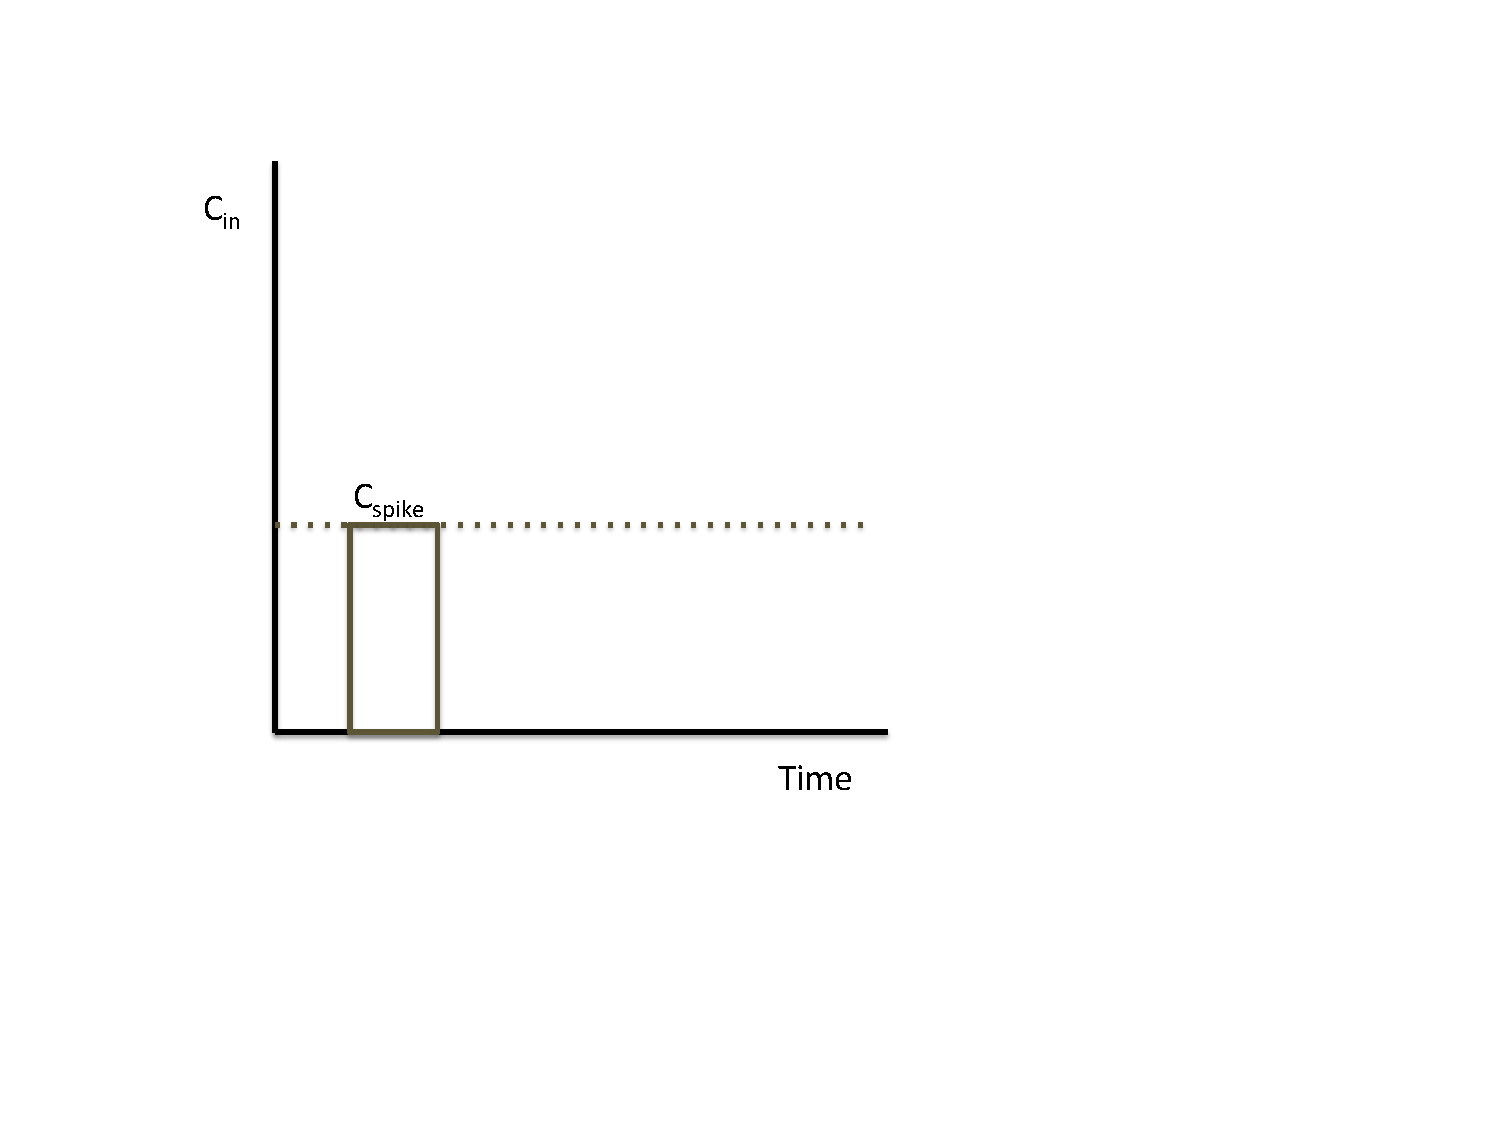
\includegraphics[width=0.4\textwidth]{C_in}
\caption{Influent concentration of a conservative tracer as a function of time.}
\end{figure}

\begin{figure}
\centering
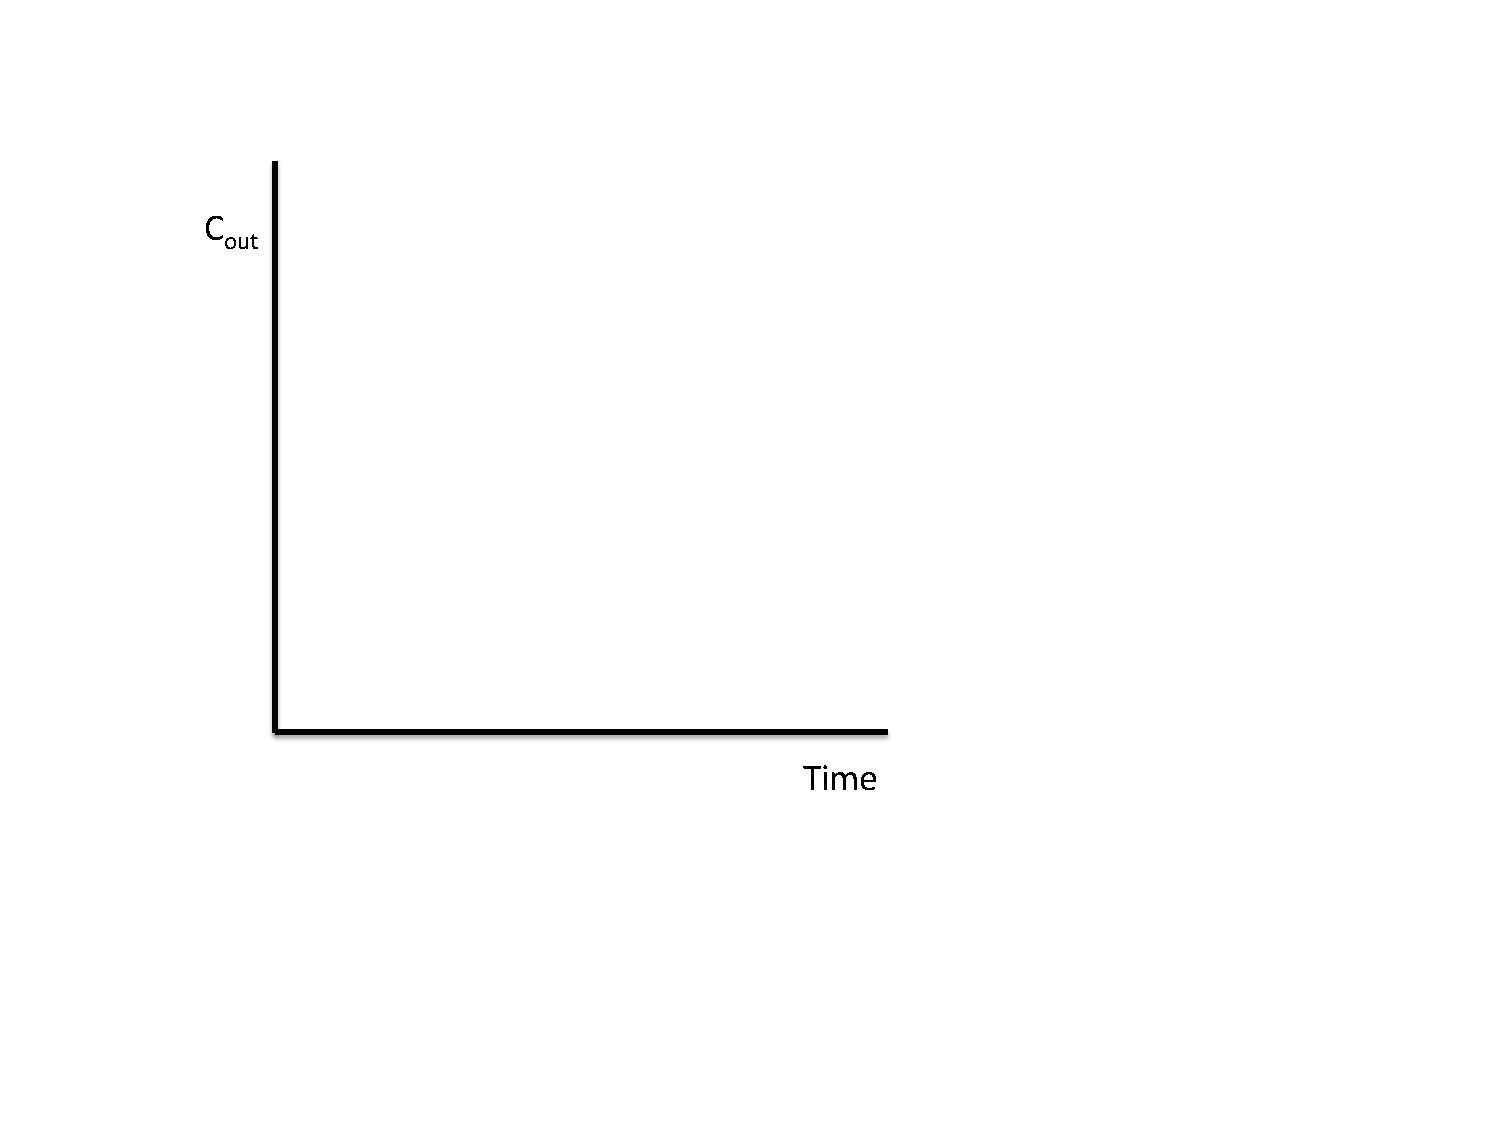
\includegraphics[width=0.4\textwidth]{C_out}
\caption{Effluent concentration of a conservative tracer from an ideal PFR as a function of time.}
\end{figure}

\begin{figure}
\centering
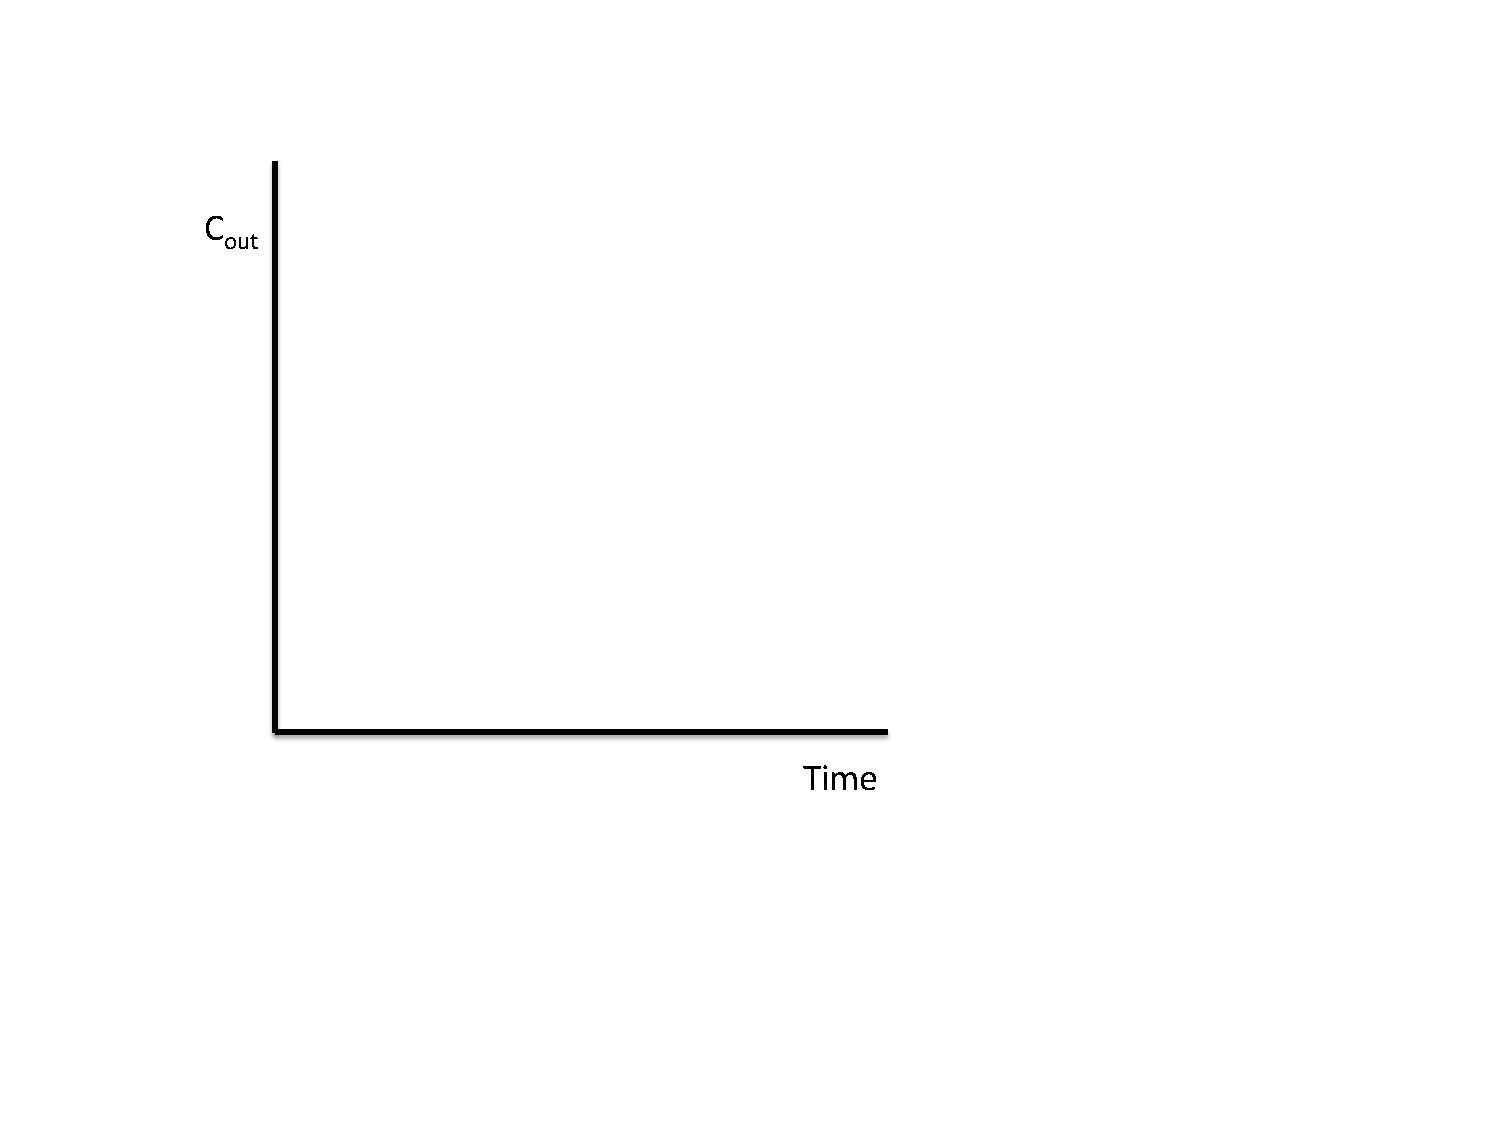
\includegraphics[width=0.4\textwidth]{C_out}
\caption{Effluent concentration of a conservative tracer from a real PFR as a function of time.}
\end{figure}

\begin{figure}
\centering
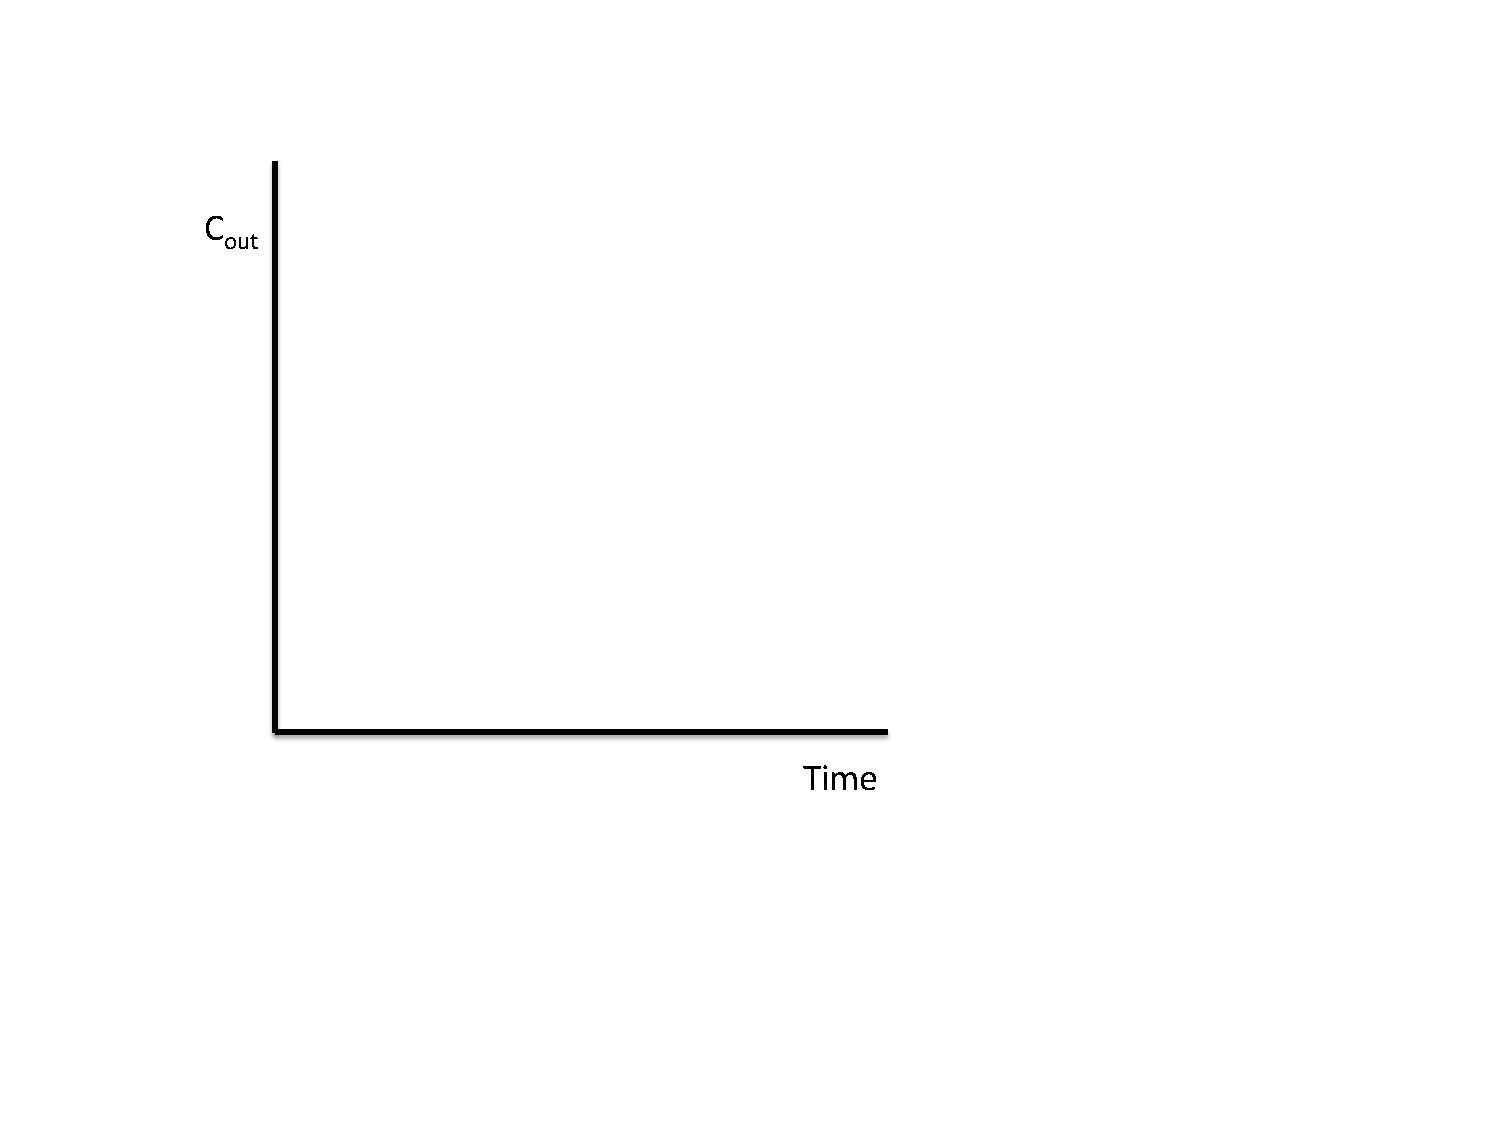
\includegraphics[width=0.4\textwidth]{C_out}
\caption{Effluent concentration of a conservative tracer from a CMFR as a function of time.}
\end{figure}



\end{document}